%\documentclass[a4paper]{article}
\documentclass[journal]{IEEEtran}

\usepackage[pdftex,pdfauthor={Shabaz Sultan, Chi Chun Wan, Boudewijn Zwaal},pdftitle={Airline sc},colorlinks=true, linkcolor=black,          % color of internal links
    citecolor=black,        % color of links to bibliography
    filecolor=black,      % color of file links
    urlcolor=black   ]{hyperref}
\usepackage[pdftex]{graphicx}
\usepackage{amsmath}
\usepackage{float}
\usepackage{listings}

\lstset{language=Python, basicstyle=\ttfamily\scriptsize, breaklines=true}

\author{Chi Chun Wan -- 2525244\\
Shabaz Sultan -- 2566703\\
Boudewijn Zwaal -- 1897527}
\title{Airline Scheduling with Simulated Annealing}
\begin{document}
\maketitle



\begin{abstract}
%\boldmath
Abstract text to go here.
\end{abstract}


\section{Introduction}
Flight schedules take up a central place in airline businesses. To maximize profit a business has to be as efficient as possible in using its resources and be as effective as possible in meeting marketplace demand. A business wants to plan its flights based on demand, use its airplanes to service these flights as efficiently as possible and assign crews to these flights to minimize expenses. These pose highly complex combinatorial optimization problems that cannot be solved analytically. Instead numerical optimization systems are used and their effectiveness can be influential on the profitability of a passenger focusses airline as a whole.\\
The Dutch airline KLM flies on 150 destinations with 97 airplanes and needs to produce a flight schedule four times a year that maximizes their profitability \cite{Bian2003}. In this paper we will consider this problem in a slightly reduced scenario, with a fictional Mokum Airways that flies on 28 destinations with 6 airplanes. The goal is to maximize profit as measured by revenue passenger kilometers, often used as unit to measure the product being sold in a passenger focussed airline \cite{Schefczyk1993}. In order to obtain the best flight schedule, we use heuristics algorithms to analyze all the possible tours and find the optimal one.\\

\section{Background}
Constructing airline schedules can be broken down in a number of subproblems, each posing a number of computational and algorithmic challenges. Often first the flights that are provided by an airline are constructed, usually subject to complex regulation and non-deterministic customer demand functions. This is referred to as the Airline Scheduling problem in the literature, where the goal is to maximize profits by meeting said demands \cite{Etschmaier1985}. \\
The next step is to assign the flights that are flown to airplanes. This is the so-called Fleet Scheduling Problem \cite{Rushmeier1997}. An airplane schedule can be constructed ahead of time, but scheduling methods for real world scenarios need to deal with real-time adjustments as well due to delays on the day itself (e.g. due to weather conditions, technical problems or issues at an airport). Ideally these schedules are repeatable (usually over either a one or seven day period), requiring that if at the start of the day an aircraft is at airport A, there needs to be an aircraft (not necessarily the exact same, just one of the same type) at airport A at the end of the schedule. \\
Finally crew personnel is assigned to the flights and airplanes. The crew scheduling problem is subject to constraints from flight authority regulation, labour regulation and airline specific regulation and because it represents the largest expenditure for airlines after fuel cost it is an important area of research for the industry as well \cite{Gopalakrishnan2005}.\\
This paper tackles the design and optimization of an airline schedule, with airplane assignment being part of the designed schedule. The one consideration given to the constraints from the crew schedule problem is that the schedule needs to have single homebase, each crew member is assumed to live at said homebase and each plane needs to attend that homebase daily for a crew change.\\
There are various approaches to this problem, such as integer programming \cite{Raff1983} or even agent based approaches \cite{Langerman1997}. One candidate for complex combinatorial optimization problems in general is Simulated Annealing \cite{kirkpatrick1983optimization}. This meta-heuristic has been applied to related problems such as crew scheduling \cite{Sosnowska2001}. It has been specifically used for airline scheduling by \cite{Mashford2001}, which is the main reference for the research described in this paper.
\section{Problem}
There are multiple formalisations of the problem to be found in the literature. We mostly follow \cite{Mashford2001}, because it most closely matches our research. Let $X$ be the set of nodes representing the airports. $G \subset X \times X$ is the service graph, making up all the valid flightpaths between two airports. In the example scenario we consider this will be the full Cartesian product between all airports, see figure~\ref{fig:service_graph}.
\\
\begin{figure}[!h]
\centering
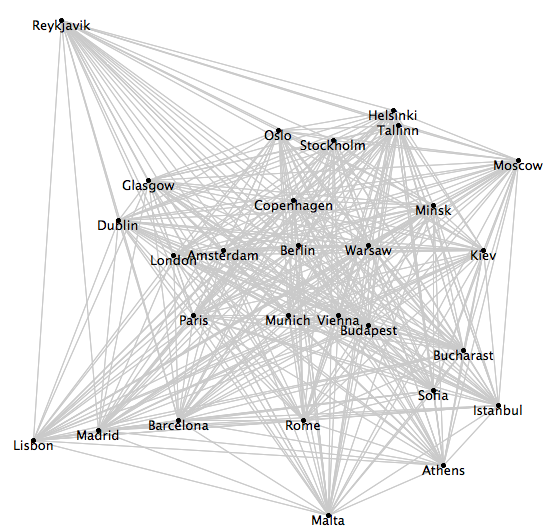
\includegraphics[width=2.3in]{service_graph}
\caption{Service graph.}
\label{fig:service_graph}
\end{figure}
\\
We schedule over an interval $[T_1, T_2]$, with $T_1 < T_2$. The fleet is defined as $F = \{p_1 \cdots p_n\}$, with $p_i$ being an airplane. The schedule for a plane is a list of flights, which are defined as quadruples $(x, y, t, p)$, with $x \in X$ the flight origin, $y \in X$ the destination, $t \in [T_1, T_2]$ the departure time and $p\in F$ the plane. \\
An airline schedule is then defined as [TODO]
\section{Algorithm}
To deal with the problem, we use two heuristic algorithms, namely hill-climbing and simulated annealing for six airplanes and one algorithm brute force for one airplane.

\subsection{Brute-force}
Brute-force is a problem-solving technique that consists of systematically enumerating all possible candidates for the solution and checking whether each candidate satisfies the problem's statement. In our case, we check all the possible tours by using a tree structure, where the node represents the destinations. A representation of the tree is given in figure~\ref{fig:tree}.\\
\begin{figure}[!h]
\centering
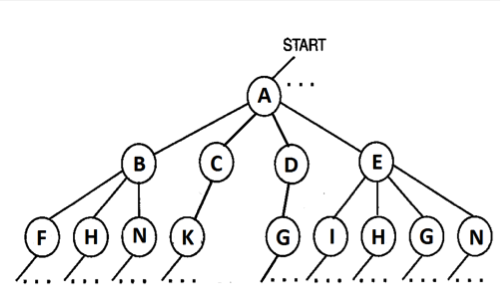
\includegraphics[width=2.5in]{tree}
\caption{Tree data structure}
\label{fig:tree}
\end{figure}
\\
An advantage of this algorithm is that the solution found, also is  the optimal solution. A disadvantage is that the run time will increases a lot to find a solution, when the state space is big. Therefore, we add branch and bound to the algorithm. The branch and bound algorithm has a upper-and lower bound. The upper bound is the theoretical maximum passengers-kilometer score and the lower bound is the best founded score so far for every step. For every position in the tree, we calculate what the maximum score is that can still be obtained from that position. If the score is lower than the current lower bound. We will not look further anymore from that position. This has as result that it will make the possibilities smaller and therefore a lower run time. 
\subsection{Hill-climbing}
Hill-climbing is an iterative algorithm that starts with an arbitrary solution to a problem, then attempts to find a better solution by changing a single element of the solution. If the change produces a better solution, an incremental change is made to the new solution, repeating until no further improvements can be found.\\
In the case of our problem, a flowchart is made in figure~\ref{fig:flowchart_hc}.\\
\begin{figure}[!h]
\centering
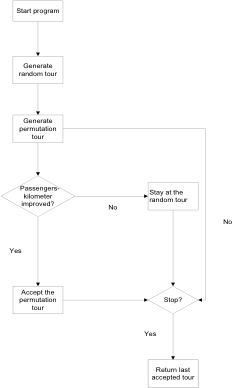
\includegraphics[width=2.5in]{flowchart_hc}
\caption{Flowchart Hill-climbing}
\label{fig:flowchart_hc}
\end{figure}
\\
\subsubsection{Tour generation and permutation}
To make hill-climbing (and later simulated annealing) work, we need a way to generate tours and to permutate these tours. The way we generate a new tour is as follows. We start in out home-base, and then we add (randomly chosen) cities to the tour until the time is full. Then from the last chosen city we generate a tree-like structure that determines all possible routes from there. If one of those routes lead us back to our home-base within the time window, we accept that one. If such a route does not exist, we cut off the last city of the generated tour and try to reach our home-base again, with the same tree-like structure. If that is not possible again, we cut off the last city one last time and try again. If it is still not possible we try it again with a whole new route. After this we check what would be the most efficient city to start (and end) in, by checking how many times we need to refuel. \\
When permutating a tour, notice that we first shift it such that our home-base is again the first city in the tour. Then we cut off a random amount of cities from the tour (except the first one, which is our home-base). We then try to create a new tour from the two endpoints created in the route. We use the same algorithm for this as we did for the generated tour, i.e. we make a tree of all possible routes from one endpoint and check if one of them leads to the other endpoint. If not we cut off a city and try it again, just as when we generate a random tour. We then again check what is the most efficient start-end city.

\subsubsection{Hill-climbing}
We start with an initial random tour generated with the algorithm described above. To find a better solution, we permutate the tour. The score of the passenger-kilometers for the initial tour is stored in a variable best score. If the score of the permutation tour is higher than the score of the arbitrary tour, the score of the permutated tour will be the new best score and the permutation tour will be accepted, otherwise the best score will stay the same and we will stay at the previous tour. This process is repeated until no further improvements can be found and the best tour is the last accepted tour. When applied to multiple planes, first one of the planes in the system is randomly chosen and its flightplan (tour) is permutated. The total score of all airplane tours is then calculated and compared to the previous best score. If it improves on said score, the new tour is accepted.\\
A disadvantage of hill-climbing is that it is good for finding a local optimum, but it is not guaranteed to find the best possible solution (global optimum). To avoid this disadvantage, we use a different algorithm, simulated annealing. \\
\subsection{Simulated Annealing}
In case of simulated annealing, it’s almost the same as hill climbing except when the solution is not improved, this solution will be accepted with a probability P. The probability is based on the number of iterations and the temperature. As the number of iterations increases, the temperature goes down and the probability will decrease. \\
In figure~\ref{fig:flowchart_sa}, the flowchart of hill-climbing is adjusted in simulated annealing.\\
\begin{figure}[!h]
\centering
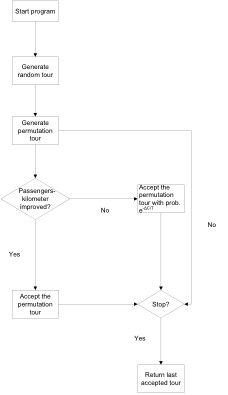
\includegraphics{flowchart_sa}
\caption{Flowchart Simulated Annealing}
\label{fig:flowchart_sa}
\end{figure}
\\
In the case when the passengers-kilometer score is not improved, you will accept the permutation tour with probability $P = e^{\frac{−\Delta C}{T}} $, where ∆C = score of the permutation tour − score of the current best tour and $T = 0, 999^i * T_0$ with $i$ is the number of iterations and $T_0$ is the start temperature 50.000.
 This probability will decrease with the number of iterations. Thus when the number of iterations increases, the temperature goes down. When temperature is high, the system will choose new states more or less at random, but as the temperature lowers this algorithm will go to hill-climbing. 
\section{Result}
To validate our method, demand and flight distances for a fictional airline are used. Mokum Airways, a newly created Dutch airline based in Amsterdam, has landing rights for 28 destinations around Europe.\\
\begin{figure}[!h]
\centering
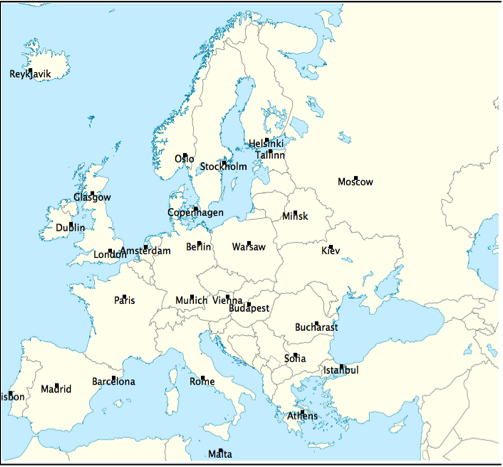
\includegraphics[width=2.5in]{europe}
\caption{Mokum Airways destinations}
\label{fig:europe}
\end{figure}
\\
\begin{figure}[!h]
\centering
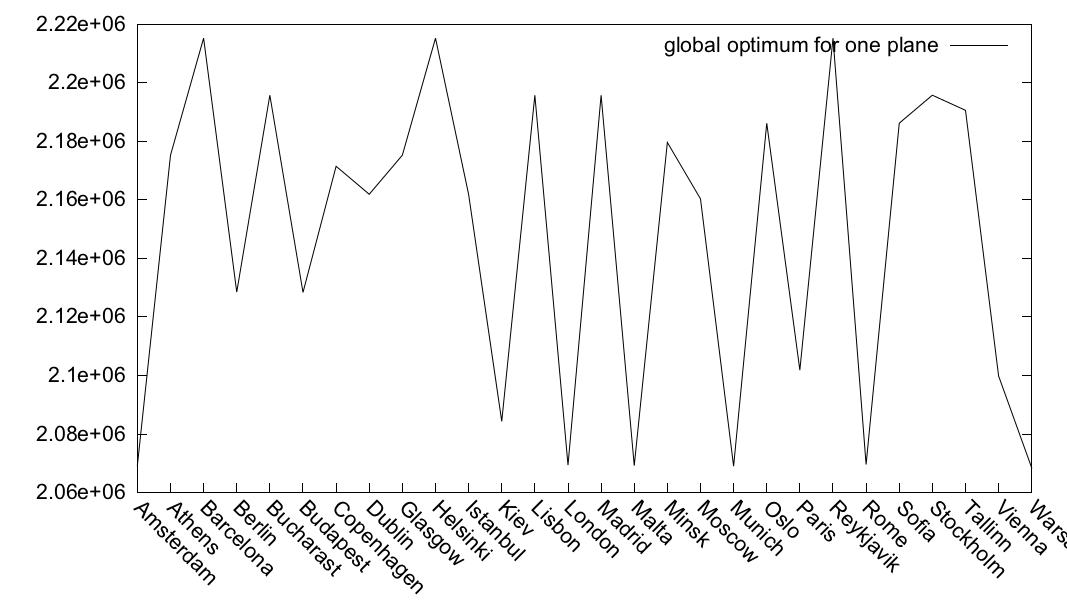
\includegraphics[width=2.5in]{different_homebases_one_plane}
\caption{Global optimum for different homebases with one plane}
\label{fig:different_homebase_one_plane}
\end{figure}
\\
The airline has a fleet of six Airbus A321 aircrafts with speed of 800km/h, capacity of 199 and range of 3199 km.  The take-off and landing take place between 02:00 and 06:00 and docking time and refuel time will take one hour. Moreover, once per day the plane needs to land in the home-base for the crew-change. The flight schedule has to be a cycle, so the start point and the end point of the route has to be the same. \\
We first tested with scheduling one airplane, to set our parameters. The results from these tests could be compared with the global optimum because we were able to use a bruteforce algorithm on the problem with one airplane. Therefore this was a good way to obtain optimal parameters, which we then used in the simulations for six airplanes too. These parameters were eventually set as follows. The cooling rate of the simulated annealing was set at 0.99999, as we found that a slow cooling gave more accurate results (although it was a bit slower). The initial temperature is set at 50.000 per plane, and thus in a simulation of six airplanes the initial temperature was 6*50.000. Then finally we terminated the simulation when more than 1000 times the accepted schedule had not changed. Of course setting this higher will results in some more accuracy, but the runtime started to get really long when we did that.  \\
One way to see if the simulated annealing was behaving properly is by looking at a graph of the score during the course of the simulation. This is shown in figure (\ref{fig:simulated_annealing_score}). We see that at first it is indeed very random, which simulated annealing is supposed to be in the beginning. Then when temperature drops to lower values the score becomes less random and will look more and more like a hill climber. Then it converges to what the simulation believes is the global optimum (although this is of course not always the case). \\
\begin{figure}[H]
\centering
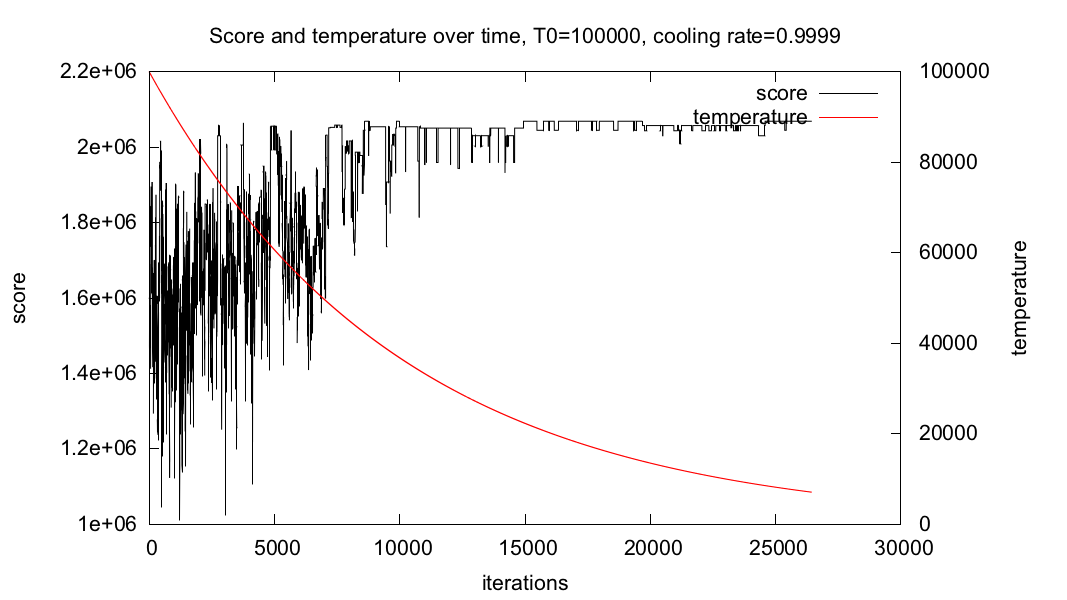
\includegraphics[width=2.5in]{score_over_time}
\caption{Score over time for Simulated Annealing}
\label{fig:simulated_annealing_score}
\end{figure}
For the results of flying with one airplane we made a plot of the best score for each home-base. This is seen in figure (\ref{fig:different_homebase_one_plane}). What we can see for instance is that Barcelona, Helsinki and Reykjavik are the best home-bases to have, having a score of 2.195.766, see figure (\ref{fig:one_plane}). If we would set Amsterdam as our home-base, which is a special case that is nice to look at (for we all live in the Netherlands), then the best score would be 2.069.202, see figure (\ref{fig:one_plane_amsterdam}). Acquiring these results took about two-three minutes per simulation.
\\
\begin{figure}[!h]
\centering
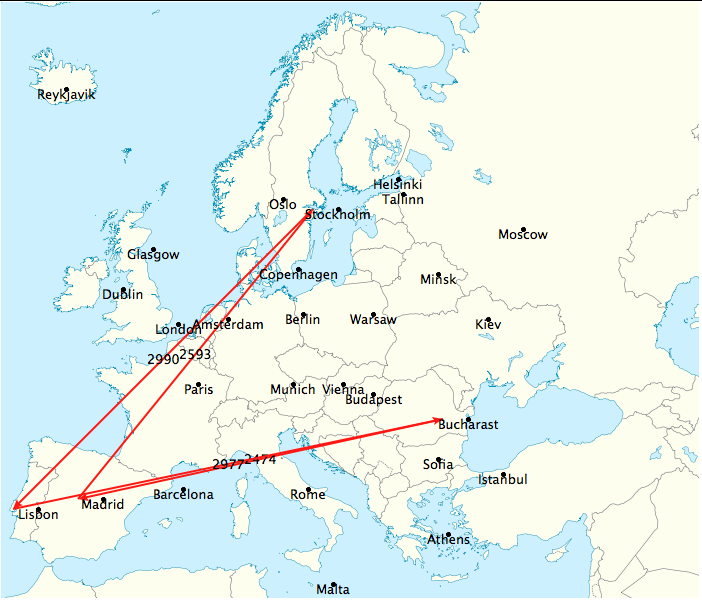
\includegraphics[width=2.5in]{best_tour_one_plane}
\caption{Best tour for one plane with any homebase, passenger kilometer score 2.215.268.}
\label{fig:one_plane}
\end{figure}
\\
\begin{figure}[!h]
\centering
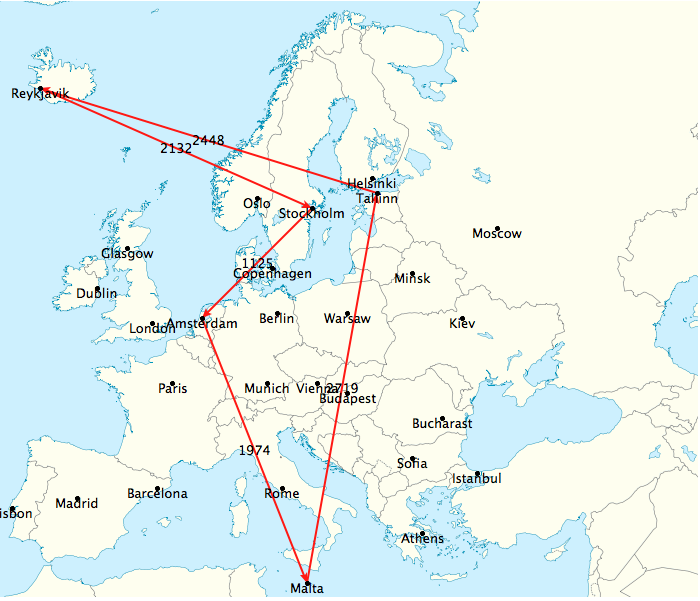
\includegraphics[width=2.5in]{best_tour_one_plane_amsterdam}
\caption{Best tour for one plane with homebase Amsterdam, passenger kilometer score 2.069.202.}
\label{fig:one_plane_amsterdam}
\end{figure}
\\
We now present the results for simulating with six airplanes. Let us begin with figure (\ref{fig:different_homebase_six_planes}). Here we see the score of both the described bruteforce algorithm as of the simulated annealer. We also see the score of what would have been if we could fly with six identical planes that fly the best route for one plane. (This is of course not possible as there are not enough passengers waiting at the gates). We can use this as a comparison, analysing this in the next section. \\
So if we set our home-base in Amsterdam, we see the best score we found with simulated annealing is 12.388.745. The highest score of all with simulated annealing is 12.892.414 with Lisbon as home-base. With our bruteforce algorithm we found an alltime highest score of 12.908.931, again with Lisbon as home-base. Acquiring these results now took about 10-30 minutes. This has a large variance but that is because of the random nature of simulated annealing.\\
What can clearly be seen is that most of the times the simulated annealer is not far off from our bruteforce approach. This indicates that our simulated annealer works quite well, further analysed in the next section. \\
\begin{figure}[!h]
\centering
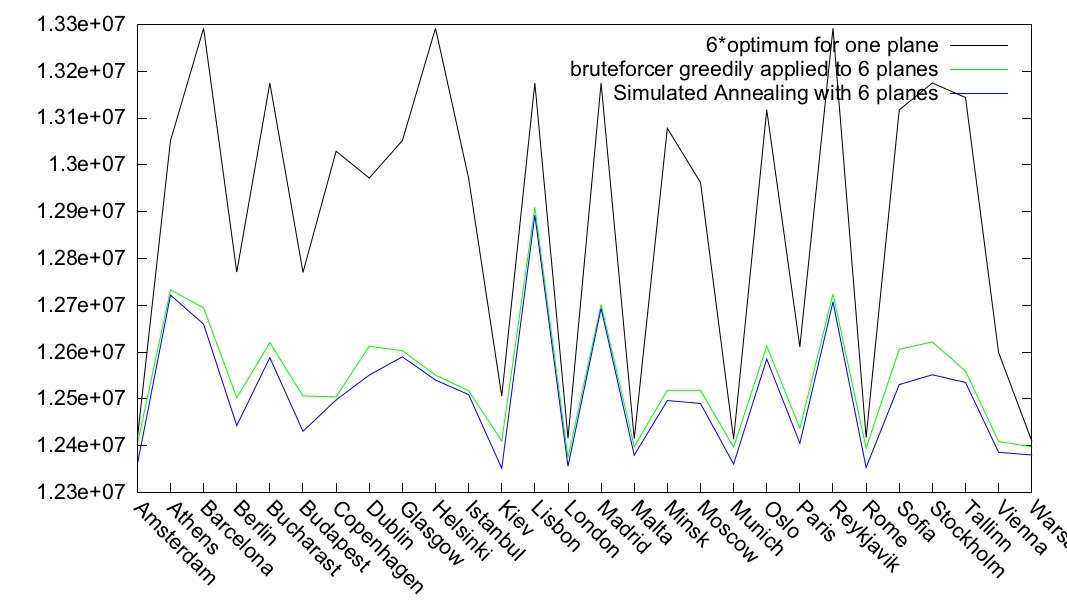
\includegraphics[width=2.5in]{different_homebases}
\caption{Results for different homebases with six planes, Simulated Annealing line based on best of 5 runs for each scenario, cooling rate of $0.99999$.}
\label{fig:different_homebase_six_planes}
\end{figure}
\\
We also have results on the average number of iterations that the simulated annealing simulation needed to find the optimum. Let us look at the following table.
\begin{lstlisting}
Average number of iterations: 328075.885714
Variance of the n.o.i.: 2025145743.66
Standard deviation of the n.o.i.: 45001.6193448
\end{lstlisting}
We see that the simulation needed quite alot of iterations before terminating. For this data we have done 5 runs per home-base for each home-base, so 5*28 runs. \\
What also can be seen is that both the algorithms have about the same peaks as the theoretical six-times-one-plane situation has. This indicates a strong correlation between these two, and thus let us estimate the behavior of six planes off the behavior of one plane.
\\
\section{Analysis}
To analyze the solution of simulated annealing. We use the result of the brute force for one airplane as reference, since the result is the global maximum. In table (1), the percentage of the global optimum found for simulated annealing is given for different cooling rates. When the decimals for the cooling rate increases, the percentage global optimum found will increase strongly, because more iterations will be run and therefore the probability to find the global optimum will be higher.
\begin{table}[h]
\begin{tabular}{ll}
Cooling Rate & Percentage global optimum found \\
0.99         & 4\%                             \\
0.999        & 6\%                             \\
0.9999       & 38\%                            \\
0.99999      & 83\%                              
\end{tabular}
\caption{\tiny{Table 1, Score one airplane SA, 100 runs, T0 = 50.000}}
\end{table}
\\
Moreover, the quality of our heuristics is tested. In figure (\ref{fig:error_sa_hc}), the RMSE of the score for simulated annealing is plotted as a black line. The number of iterations depends on the cooling rate, a lower cooling rate will increase the number of iterations and thereby the run time. However, the RMSE  decreases with the number of iterations. Thus, the result will be more accurate. 
\\
\\
To analyze the two heuristics, hill climbing and simulated annealing, we can look at the same figure (\ref{fig:error_sa_hc}) for both heuristics for the same iterations against the RMSE. The RMSE for the same iteration for the hill climber is  higher than the simulated annealing. Thus, the simulated annealing is in this case better for finding the optimal solution than the hill climbing, since the risk to get into a local optimum is limited. 
\\
\\
An interesting analysis is whether the solution for one airplane can predict the solution for six airplanes. In figure (\ref{fig:different_homebase_six_planes}), the score times 6 for one airplane follows almost the same pattern as the score of the simulated annealing for six airplanes for different home bases. We ran a correlation test. This resulted in a correlation coefficient of 0.820 for simulated annealing. Therefore, we can conclude there is a correlation between the prediction for the score of six airplanes when the score for one airplane is known. 
\\
\\

\begin{figure}[H]
\centering
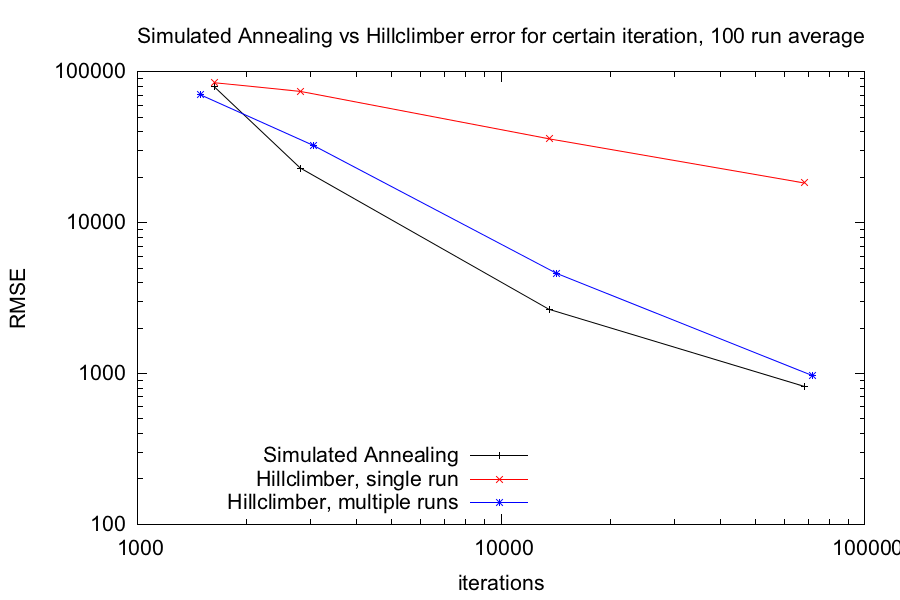
\includegraphics[width=2.5in]{iterations_vs_error_sa_hc}
\caption{Error for Simulated Annealing and Hill-climbing.\tiny}
\label{fig:error_sa_hc}
\end{figure}
\section{Conclusions}
In conclusion we can say that our simulated annealer works very well. After analyzing the various results we see that compared to the bruteforcer our simulated annealer performs very close to it. Also with a runtime of between 10 and 30 minutes to find an optimal schedule for six airplanes, it is not all that slow. Of course one can do the simulation faster, but we showed that the accuracy of the results then will decline.\\ 
We can conclude as well that the simulated annealer works better than the hill climber, as discussed in the analysis section.
We also showed that the outcome of scheduling six airplanes can be predicted with the output of the simulation with one plane. We found a high correlation between the global optimum of one airplane and the global optimum of six airplanes, and this can be seen also in figure (\ref{fig:different_homebase_six_planes}), as the peaks agree of both sources. [IMPROVEMENTS?]\\

\bibliographystyle{IEEEtran}
\bibliography{final_report}
\end{document}

